%\begin{document}

\begin{figure*}[t]
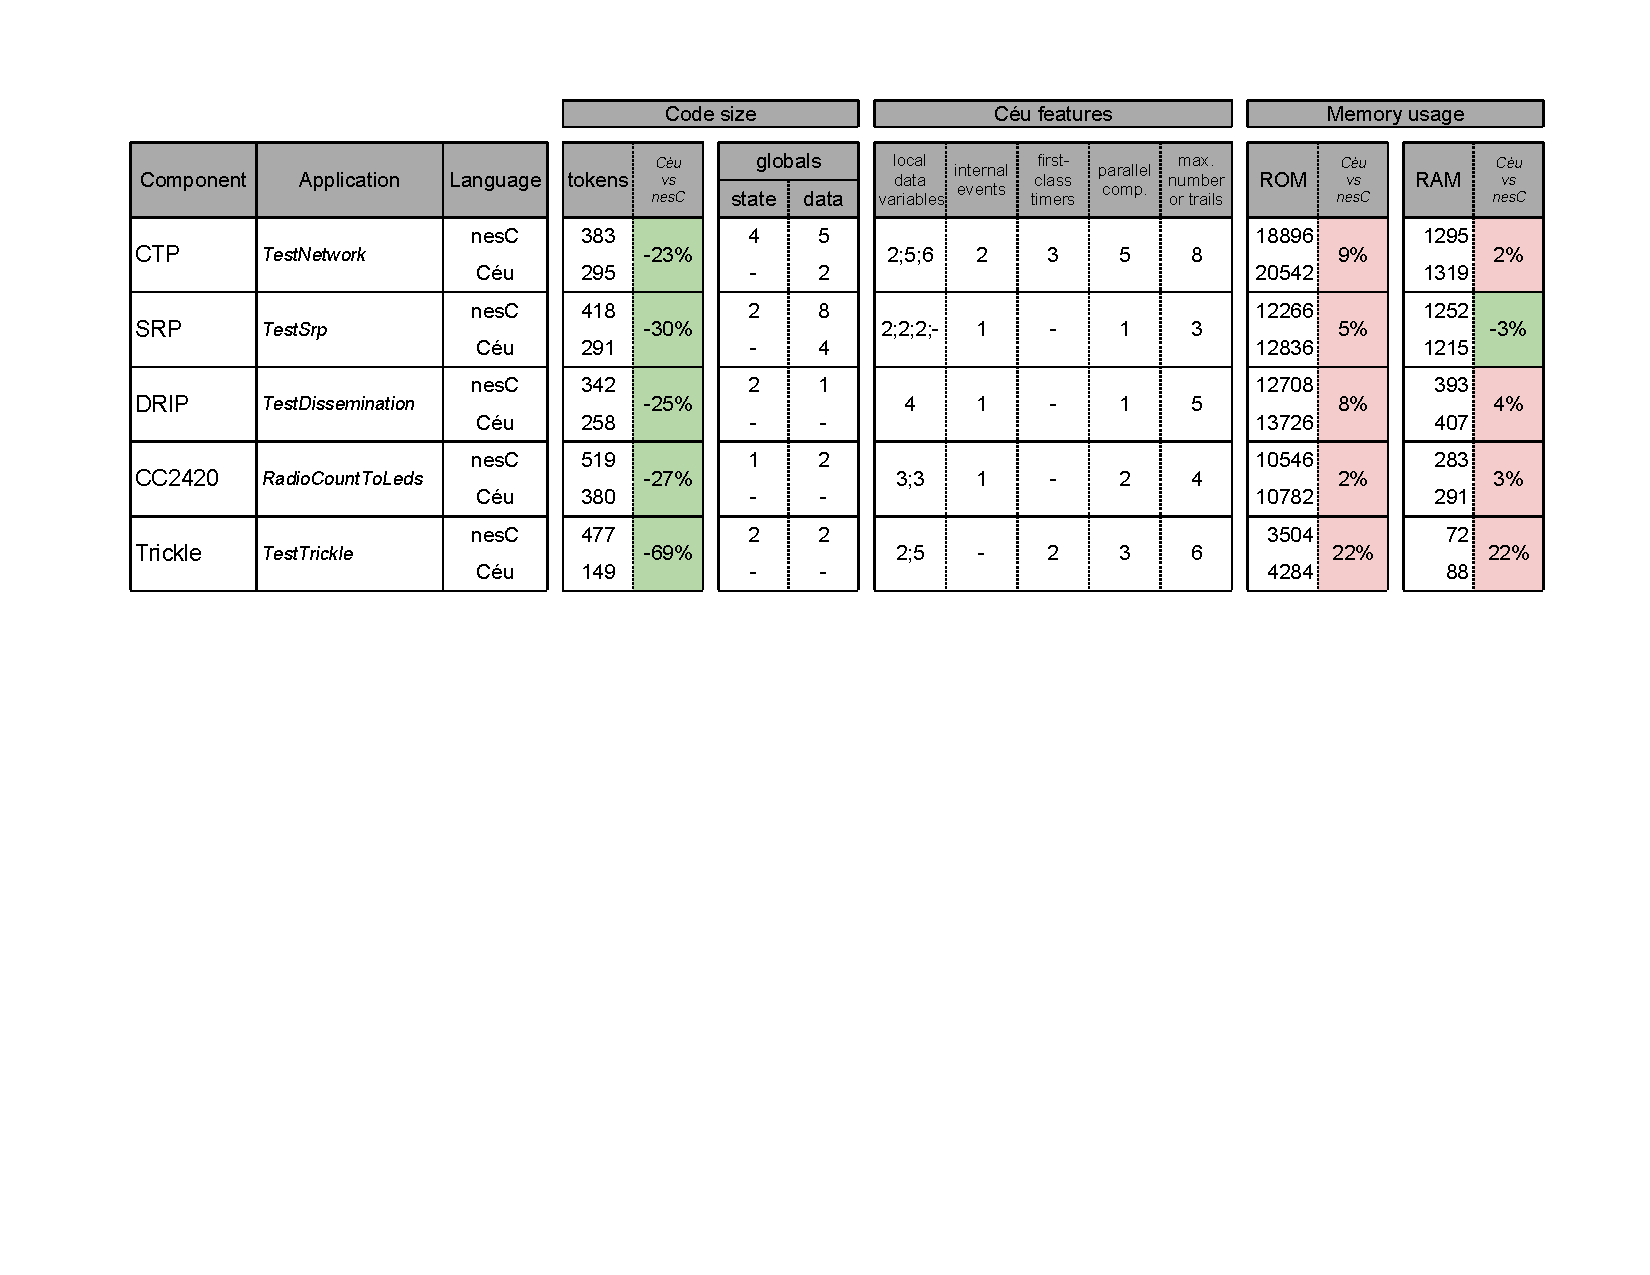
\includegraphics[width=\textwidth]{eval}
%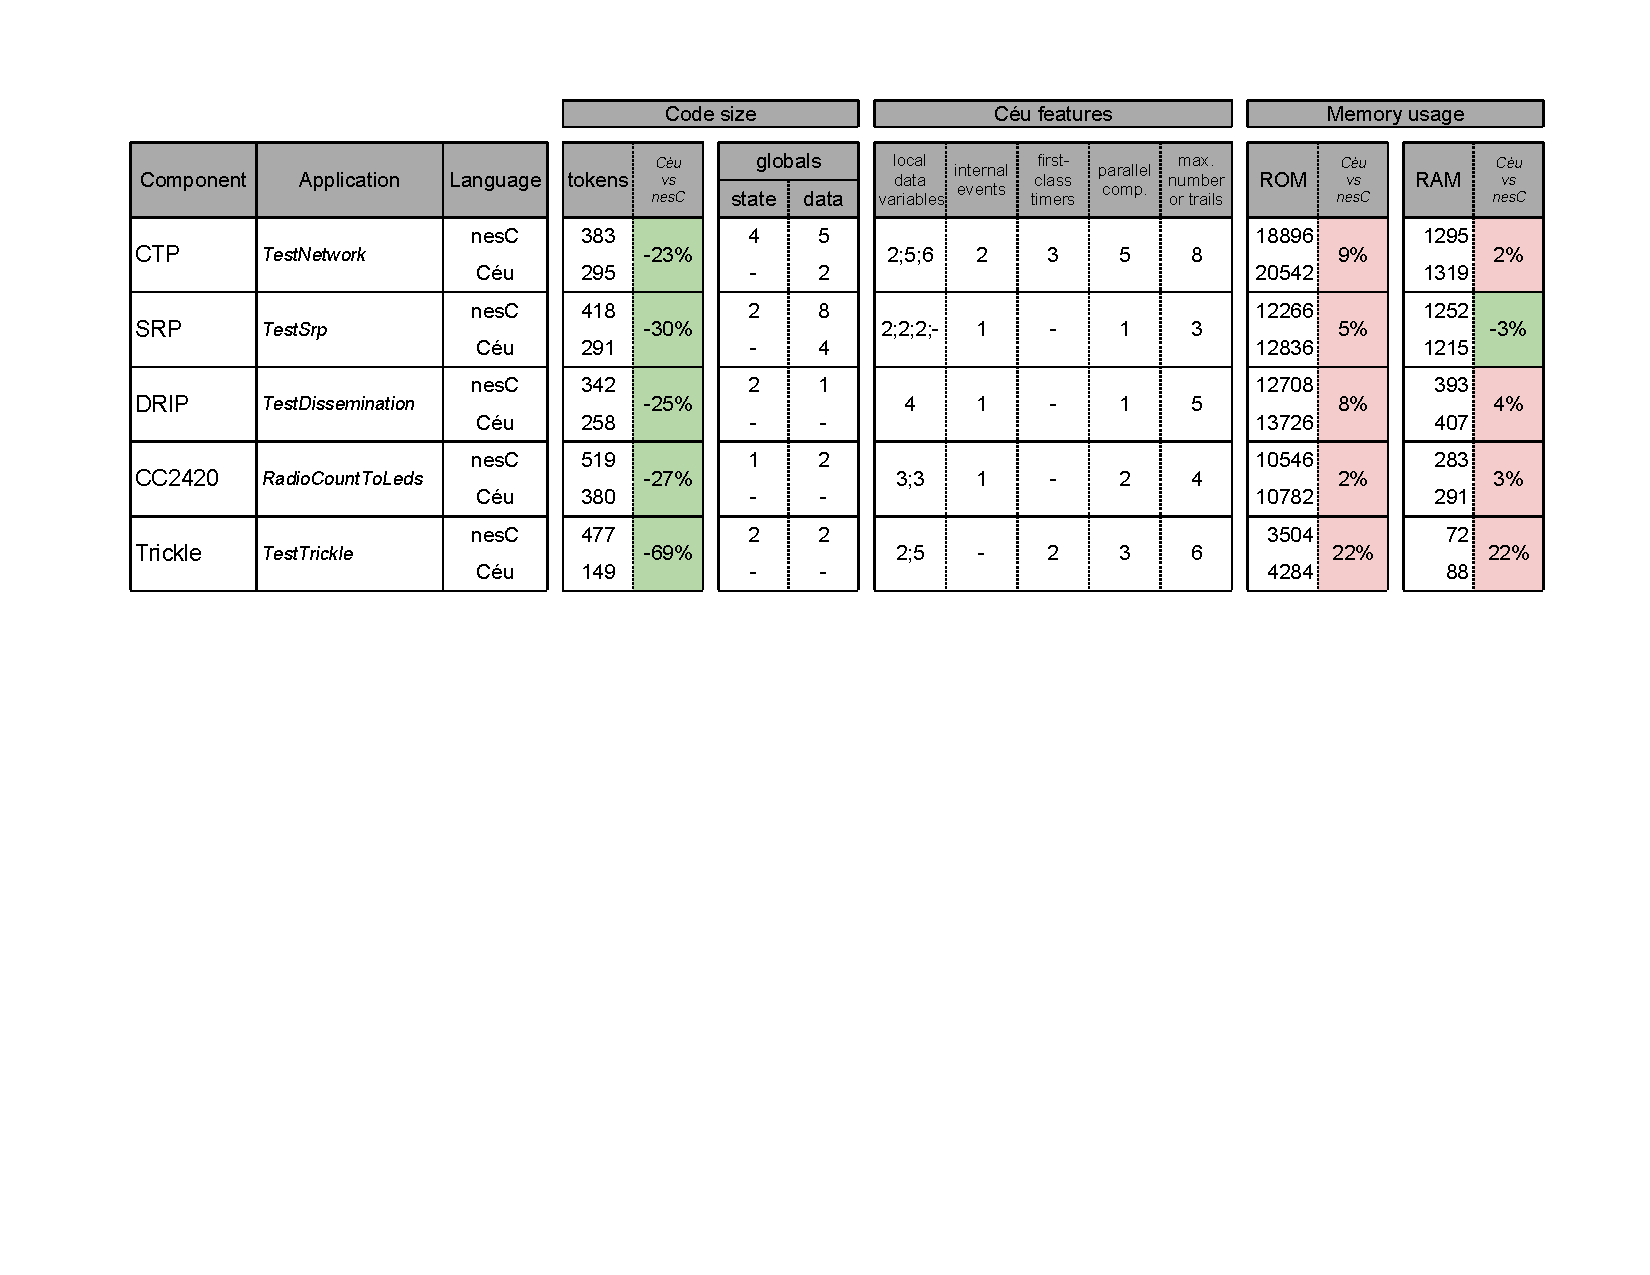
\includegraphics{eval}
\caption{ Comparison between \CEU and \emph{nesC} for the implemented 
applications. \newline
{\small %\textmd{
The column group \emph{Code size} compares the number of language tokens and 
global variables used in the sources;
the group \emph{C\'eu features} shows the number of times each functionality is 
used in each application;
the group \emph{Memory usage} compares ROM and RAM consumption.
}%}
\label{fig.eval}
}
\end{figure*}

In this chapter we present a quantitative evaluation of \CEU.
%
Our assumption is that when considering \CEU for system-level development, 
programmers would face a tradeoff between code simplicity and efficient 
resource usage.
%
For this reason, we evaluate source code size, memory usage, event-handling 
responsiveness, and battery consumption for a number of standardized protocols 
in TinyOS~\cite{wsn.teps}.
%
We use code size as a metric for code simplicity, complemented with a 
qualitative discussion regarding the eradication of explicit state variables 
for control purposes.
%
By responsiveness, we mean how quickly programs react to incoming events (to 
avoid missing them).
%
Memory, responsiveness are important resource-efficiency measures to evaluate 
the negative impact with the adoption of a higher-level language.
%
In particular, responsiveness (instead of total CPU cycles) is a critical 
aspect in reactive systems, specially those with a synchronous execution 
semantics where preemption is forbidden.
%
We also discuss battery consumption when evaluating responsiveness.

Our criteria to choose which language and applications to compare with \CEU are 
based on the following guidelines:
%
\begin{itemize}
\item Compare to a resource-efficient programming language in terms of memory 
and speed.
\item Compare to the best available codebase, with proved stability and 
quality.
\item Compare relevant protocols in the context of WSNs.
\item Compare the control-based aspects of applications, as \CEU is designed 
      for this purpose.
\item Compare the radio behavior, the most critical and battery-drainer 
      component in WSNs.
\end{itemize}
%
Based on these criteria, we chose \emph{nesC} as the language to compare, given 
its resource efficiency and high-quality codebase%
\footnote{TinyOS repository: \url{http://github.com/tinyos/tinyos-release/}}.
%
In addition, \nesc is used as benchmark in many systems related to 
\CEU~\cite{wsn.protothreads,wsn.sol,wsn.ocram,wsn.flowtalk}.
In particular, the work on \emph{Protothreads}~\cite{wsn.protothreads} is a 
strong reference in the WSN community, and we adhere to similar choices in our 
evaluation.
%
All chosen applications are reference implementations of open standards in the 
TinyOS community~\cite{wsn.teps}:
the receiving component of the \emph{CC2420} radio driver;
the \emph{Trickle} timer;
the \emph{SRP} routing protocol;
the \emph{DRIP} dissemination protocol;
and the routing component of the \emph{CTP} collection protocol.
%
They are representative of the realm of system-level development for WSNs, 
which mostly consists of network protocols and low-level system utilities:
%
%Justifying each choice individually,
a radio driver is mandatory in the context of WSNs;
the trickle timer is used as a service by other important
protocols~\cite{wsn.trickle,wsn.ctp};
routing, dissemination, and collection are the most common classes of protocols 
in WSNs.

%TTT drip vs dip
%Although DRIP is simpler than other dissemination alternatives~\cite{wsn.dip, 
%wsn.}, they mostly vary on , and we chose the smallest available 
%implementation in \emph{nesC} of each.
%
%The (e.g. DIP

We took advantage of the component-based model of TinyOS and all of our 
implementations use the same interface provided by the \emph{nesC} counterpart.
This approach has two advantages:
first, we could reuse existing applications in the TinyOS repository to test 
the protocols (e.g. \emph{RadioCountToLeds} or \emph{TestNetwork});
second, sticking to the same interface forced us to retain the original 
architecture and functionality, which also strengths our evaluation.

Figure~\ref{fig.eval} shows the comparison for \emph{Code size} and 
\emph{Memory usage} between the implementations in \emph{nesC} and \CEU.
%
For memory usage, detailed in Section~\ref{sec.eval.resource}, we compare the 
binary code size and required RAM.
%
For code size, detailed in Section~\ref{sec.eval.code}, we compare the number 
of tokens used in the source code.
%The figure also details how many times each relevant feature of \CEU was used 
%in the implementations, helping to identify the patterns that reduce the code 
%size (to be discussed further).
%
For responsiveness, detailed in Section~\ref{sec.eval.radio}, we evaluate the 
capacity to promptly acknowledge radio packet arrivals in the $CC2420$ driver.

\section{Code size}
\label{sec.eval.code}

We use two metrics to compare code complexity between the implementations in 
\CEU and \emph{nesC}: the number of language tokens and global variables used 
in the source code.
%
Similarly to comparisons in related work~\cite{wsn.ocram,wsn.protothreads}, we 
did not consider code shared between the \emph{nesC} and \CEU implementations 
(e.g. predicates, \code{struct} accessors, etc.), as they do not represent 
control functionality and pose no challenges regarding concurrency aspects.

%We chose to use tokens instead of lines of code because code density in \CEU 
%is considerably lower, given that most lines are composed of a single block 
%delimiter from a structural composition.
%
Note that the languages share the core syntax for expressions, calls, and field 
accessors (based on $C$), and we removed all verbose annotations from the 
\emph{nesC} implementations for a fair comparison (e.g. \code{signal}, 
\code{call}, \code{command}, etc.).
%
The column \emph{Code size} in Figure~\ref{fig.eval} shows a considerable 
decrease in the number of tokens for all implementations (around at least 
25\%).

Regarding the metrics for number of globals, we categorized them in 
\emph{state} and \emph{data} variables.

State variables are used as a mechanism to control the application flow (on the 
lack of a better primitive).
Keeping track of them is often regarded as a difficult task, hence, reduction 
of state variables has already been proposed as a metric of code complexity in 
a related work~\cite{wsn.protothreads}.
The implementations in \CEU, not only reduced, but completely eliminated state 
variables, given that all control patterns could be expressed with hierarchical 
compositions of activities assisted by internal-event communication.

Data variables in WSN programs usually hold message buffers and protocol 
parameters (e.g. sequence numbers, timer intervals, etc.).
In event-driven systems, given that stacks are not retained across reactions to 
the environment, all data variables must be global%
\footnote{In the case of \emph{nesC}, we refer to globals as all variables 
defined in the top-level of a component implementation block, which are visible 
to all functions inside it.}.
Although the use of local variables does not imply in reduction of lines of 
code (or tokens), the smallest the scope of a variable, the more readable and 
less susceptible to bugs the program becomes.
%
In the \CEU implementations, most variables could be nested to a deeper scope.
The column \emph{local data variables} in Figure~\ref{fig.eval} shows the depth 
of each new local variable in \CEU that was originally a global in \emph{nesC} 
(e.g. ``2;5;6'' represents globals that became locals inside blocks in the 2nd, 
5th, and 6th depth level).

The columns under \emph{C\'eu features} in Figure~\ref{fig.eval} point out how 
many times each functionality has been used in the implementations in \CEU, 
helping to identify where the reduction in size comes from.
%
As an example, Trickle uses 2 timers and 3 parallel compositions, resulting in 
at most 6 trails active at the same time.
% (a \code{par} may spawn more than 2 trails).
The use of six coexisting trails for such a small application is justified by 
its highly control-intensive nature, and the almost 70\% code reduction 
illustrates the huge gains with \CEU in this context.
% TODO: what about CTP? (roberto)
%
%TODO: CTP c/ select

% TODO: DRIP uses trickle as a service (does not implement it)

\section{Memory usage}
\label{sec.eval.resource}

Memory is a scarce resource in motes and it is important that \CEU does not 
pose significant overheads in comparison to \emph{nesC}.
%
We evaluate ROM and RAM consumption by using available testing applications for 
the protocols in the TinyOS repository.
%They were carefully tweaked to generate a minimal binary that tests only the 
%components of interest.
Then, we compiled each application twice: first with the original component in 
\emph{nesC}, and then with the new component in \CEU.
%
Column \emph{Memory usage} in Figure~\ref{fig.eval} shows the consumption of 
ROM and RAM for the generated applications.
With the exception of the Trickle timer, the results in \CEU are below 10\% in 
ROM and 5\% in RAM, in comparison with the implementations in \emph{nesC}.
%
Our method and results are similar to those for
Protothreads~\cite{wsn.protothreads}, which is an actively supported 
programming system for the Contiki OS~\cite{wsn.contiki}.
% with a simple and lightweight implementation based on a set of C macros.

Note that the results for Trickle illustrate the footprint of the runtime of 
\CEU.
The RAM overhead of 22\% actually corresponds to only 16 bytes: 1 byte for each 
of the maximum 6 concurrent trails, and 10 bytes to handle synchronization 
among timers.
%
As the complexity of the application grows, this basic overhead tends to become 
irrelevant.
%
The SRP implementation shows a decrease in RAM, which comes from the internal 
communication mechanism of \CEU that could eliminate a queue.
%
Note that both TinyOS and \CEU define functions to manipulate queues for timers 
and tasks (or trails).
Hence, as our implementations use components in the two systems, we pay an 
extra overhead in ROM for all applications.

We focused most of the language implementation efforts on RAM optimization, as 
it has been historically considered more scarce than ROM~\cite{wsn.decade}.
Although we have achieved competitive results, we expected more gains with 
memory reuse for blocks with locals in sequence, because it is something that 
cannot be done automatically by the \emph{nesC} compiler.
However, we analyzed each application and it turned out that we had no gains 
\emph{at all} from blocks in sequence.
Our conclusion is that sequential patterns in WSN applications come either from 
split-phase operations, which always require memory to be preserved (between 
the request and the answer);
or from loops, which do reuse all memory, but in the same way that event-driven 
systems do.

\section{Responsiveness}
\label{sec.eval.radio}

A known limitation of languages with synchronous and cooperative execution is 
that they cannot guarantee hard real-time 
deadlines~\cite{wsn.comparison,wsn.tosthreads}.
%
For instance, the rigorous synchronous semantics of \CEU forbids 
non-deterministic preemption to serve high priority trails.
%
Even though \CEU ensures bounded execution for reactions, this guarantee is not 
extended to $C$ function calls, which are usually preferred for executing long 
computations (due to performance and existing code base).
%
%Even though WSN protocols are usually tolerant to faults (given the unreliable 
%link), packet losses affect the network performance and cause motes to spend 
%more battery.
%
The implementation of a radio driver purely in \CEU raises questions
regarding its responsiveness, therefore, we conduct two experiments in this 
section.
% in order to evaluate it.
%
The experiments use the \emph{COOJA} simulator~\cite{wsn.cooja} running images 
compiled to \emph{TelosB} motes.

In the first experiment, we ``stress-test'' the radio driver to compare its 
performance in the \CEU and \emph{nesC} implementations.
We use 10 motes that broadcast 100 consecutive packets of 20 bytes to a mote 
that runs a periodic time-consuming activity.
The receiving handler simply adds the value of each received byte to a global 
counter.
% (we set a single random byte for each packet, so that the sum is always 1).
%
The sending rate of each mote is 200ms (leading to a receiving average of 50 
packets per second considering the 10 motes), and the time-consuming activity 
in the receiving mote runs every 140ms.
%
Note that these numbers are much above typical WSN applications: 10 neighbours 
characterizes a dense topology; 20 bytes plus header data is close to the 
default limit for a TinyOS packet; and 5 messages per second is a high 
frequency on networks that are supposedly idle most of the time.
%
We run the experiment varying the duration of the lengthy activity from 1 to 
128 milliseconds, covering a wide set of applications (summarized in 
Table~\ref{tab.durs}).
%
We assume that the lengthy operation is implemented directly in $C$ and cannot 
be easily split in smaller operations (e.g., recursive 
algorithms~\cite{wsn.comparison,wsn.tosthreads}).
So, we simulated them with simple busy waits that would keep the driver in \CEU 
unresponsive during that period.
%(given the run completion semantics of the language).
%We certified that the operation executed the same number of times in \CEU and 
%\emph{nesC} for all tests in the experiment.

Figure~\ref{fig.radio1} shows the percentage of handled packets in \CEU and 
\emph{nesC} for each duration.
%
Starting from the duration of 6ms for the lengthy operation, the responsiveness 
of \CEU degrades in comparison to \nesc (5\% of packet loss).
%every 140ms, while receiving a new packet every 20ms
%
The \emph{nesC} driver starts to become unresponsive with operations that take 
32ms, which is a similar conclusion taken from TOSThreads experiments with the 
same hardware~\cite{wsn.tosthreads}.
%
\begin{comment}
Our direct interpretation is that the \CEU driver starts to become unresponsive 
when receiving packets every 20ms while executing a periodic operation of 16ms 
(which is keeping the CPU unresponsive 80\% of the time).
The same interpretation can be done for \emph{nesC}, but considering a 64-ms 
operation,
\end{comment}
%
Table~\ref{tab.durs} shows the duration of some lengthy operations specifically 
designed for WSNs found in the literature.
The operations in the group with timings up to $6ms$ could be used with 
real-time responsiveness in \CEU (considering the proposed high-load 
parameters).
%a 5\% decrease in performance in comparison with \emph{nesC}.

\begin{figure}[t]
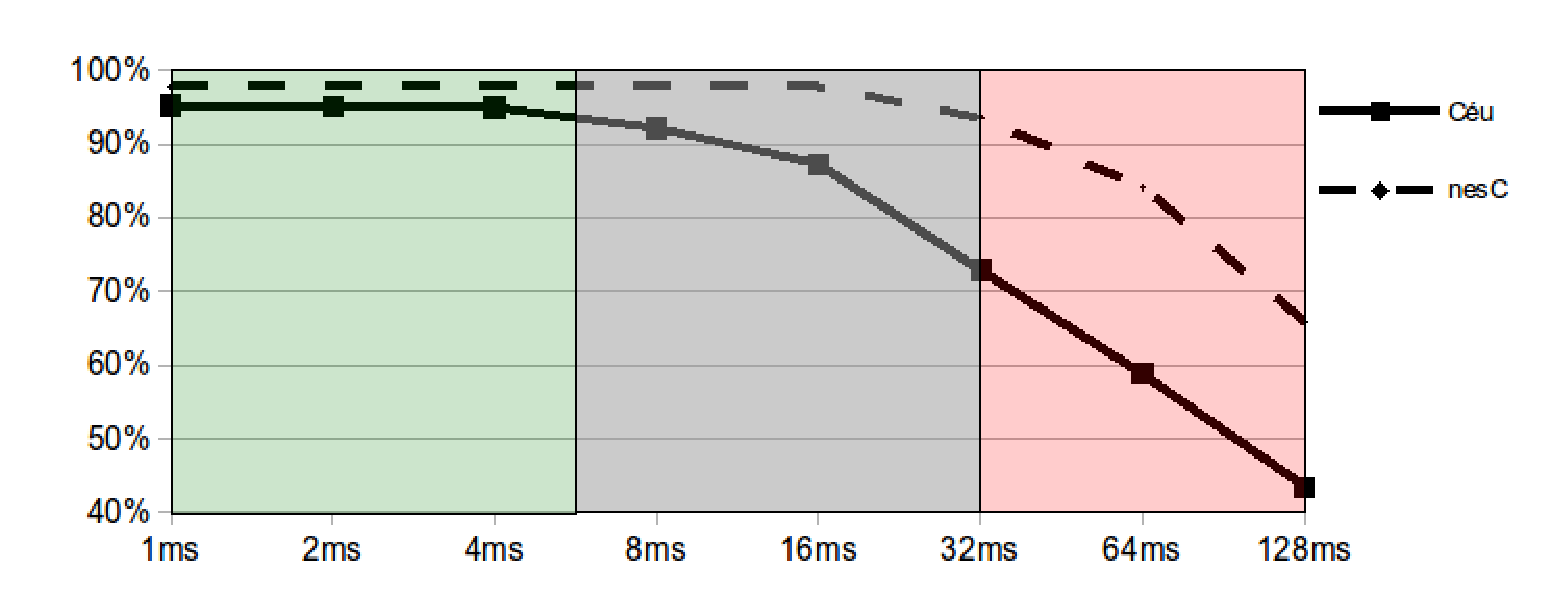
\includegraphics[width=\linewidth,clip=true,trim=5px 0px 5px 0px]{radio1}
%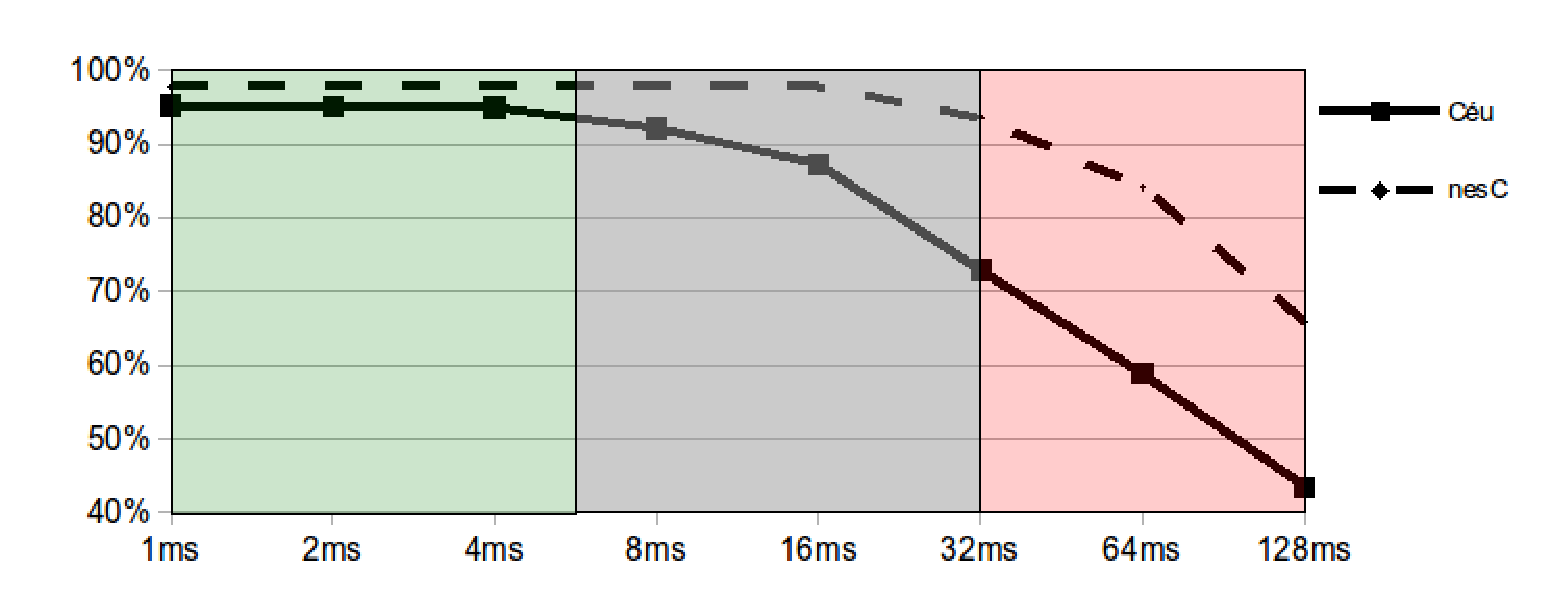
\includegraphics[width=\linewidth,clip=true,trim=35px 0px 10px 0px]{radio1}
%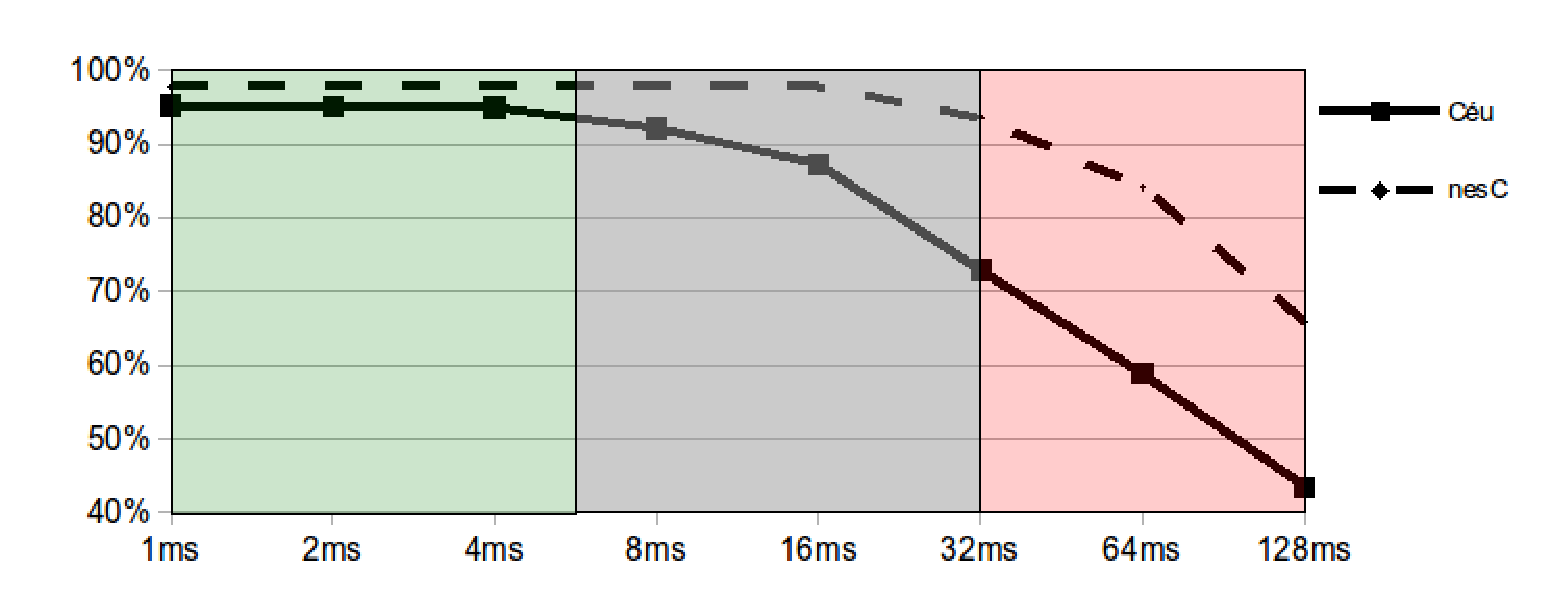
\includegraphics{radio1}
\caption{ Percentage of received packets depending on the duration of the 
lengthy operation.  \newline
{\small %\textmd{
Note the logarithmic scale on the \emph{x}-axis.
The packet arrival frequency is 20ms.
The operation frequency is 140ms.
%Starting from a 16-ms duration, \CEU performs 5\% worse than \emph{nesC}.
In the (left) green area, \CEU performs similarly to \emph{nesC}.
The (middle) gray area represents the region in which \emph{nesC} is still 
responsive.
In the (right) red area, both implementations become unresponsive (i.e. over 
5\% packet losses).
}%}
\label{fig.radio1}
}
\end{figure}

\definecolor{lightgreen}{rgb}{.8,1,0.8}
\definecolor{lightred}{rgb}{1,.8,.8}
\definecolor{darkgray}{rgb}{.66,.66,.66}

\begin{table}[t]
\begin{center}
\begin{tabular}{ | l | r | }
\hline
\rowcolor{darkgray}
    Operation          & Duration  \\ \hline
\hline
\rowcolor{lightgreen}
    Block cypher~\cite{wsn.tinysec,wsn.crypto}  & 1ms           \\ \hline
\rowcolor{lightgreen}
    MD5 hash~\cite{wsn.crypto}                  & 3ms           \\ \hline
\rowcolor{lightgreen}
    Wavelet decomposition~\cite{wsn.wavelet}    & 6ms           \\ \hline
\hline
\rowcolor{lightred}
    SHA-1 hash~\cite{wsn.crypto}                & 8ms           \\ \hline
\rowcolor{lightred}
    RLE compression~\cite{wsn.compression}      & 70ms          \\ \hline
\rowcolor{lightred}
    BWT compression~\cite{wsn.compression}      & 300ms         \\ \hline
\rowcolor{lightred}
    Image processing~\cite{wsn.cyclops}         & 50--1000ms    \\ \hline
\end{tabular}
\caption{Durations for lengthy operations is WSNs. \newline
{\small %\textmd{
\CEU can perform the operations in the green rows in real-time and under high 
loads.
}%}
\label{tab.durs}
}
\end{center}
\end{table}

Although we did not perform specific tests to evaluate CPU usage, the 
experiment suggests that the overhead of \CEU over \emph{nesC} is very low.
%
When the radio driver is the only running activity (column $1ms$, which is the 
same result for an addition test we did for $0ms$), both implementations loose 
packets with a difference under 3 percentage points.
This difference remains the same up to 4-ms activities, hence, the observed 
degradation for longer operations is only due to the lack of preemption, not 
execution speed.
%
Note that for lengthy operations implemented in $C$, there is no runtime 
overhead at all, as the generated code is the same for \CEU and \emph{nesC} 
(i.e. \CEU and \emph{nesC} just call $C$).

In the second experiment, instead of running a long activity in parallel, we 
use a 8-ms operation tied in sequence with every packet arrival to simulate an 
activity such as encryption.
We now run the experiment varying the rate in the 10 sending motes from 600ms 
to 100ms (i.e., 60ms to 10ms receiving rate if we consider the 10 motes).
%
Figure~\ref{fig.radio2} shows the percentage of handled packets in \CEU and 
\emph{nesC} for each rate of message arrival.
%
%The last column shows the theoretical limit of 80ms (i.e., receiving a packet 
%every 8ms and handling it in 8ms).
%
The results show that \CEU is 100\% responsive up to frequency of 33 packets 
per second, while \emph{nesC} up to 50 packets.

\begin{figure}[t]
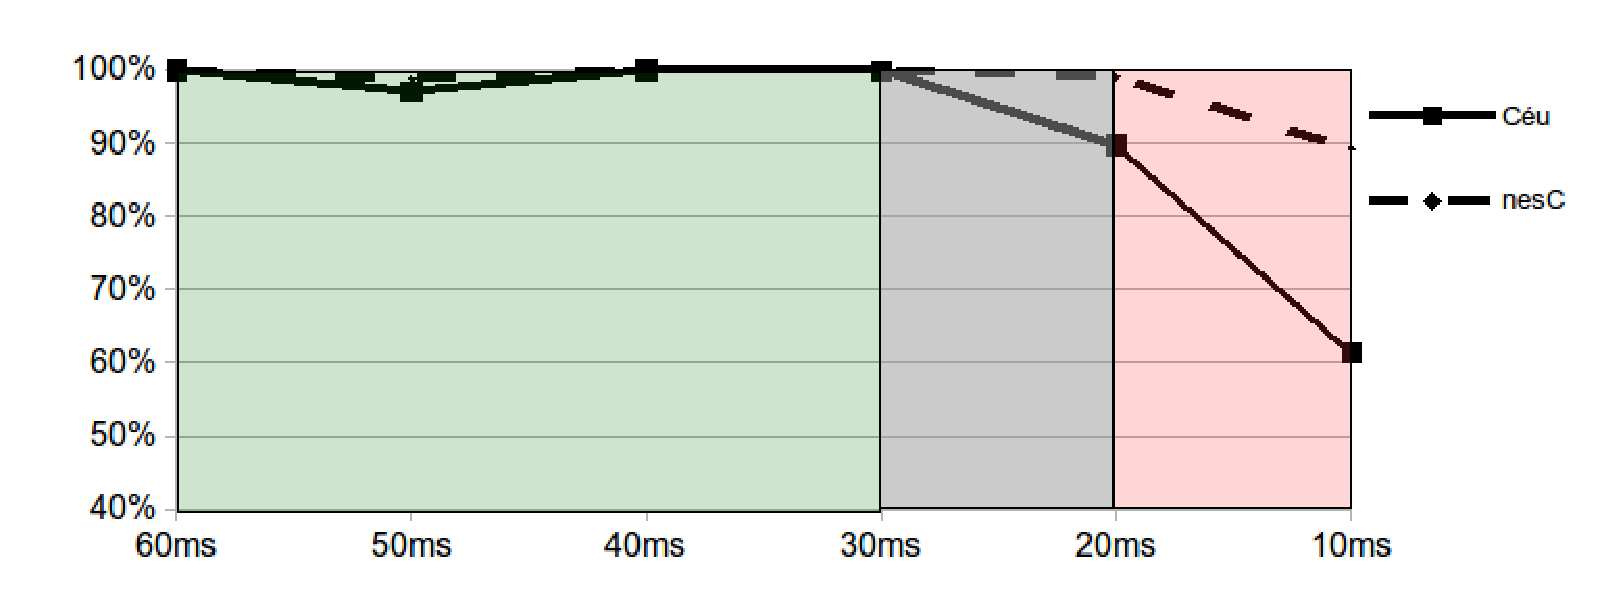
\includegraphics[width=\linewidth,clip=true,trim=5px 0px 5px 0px]{radio2}
%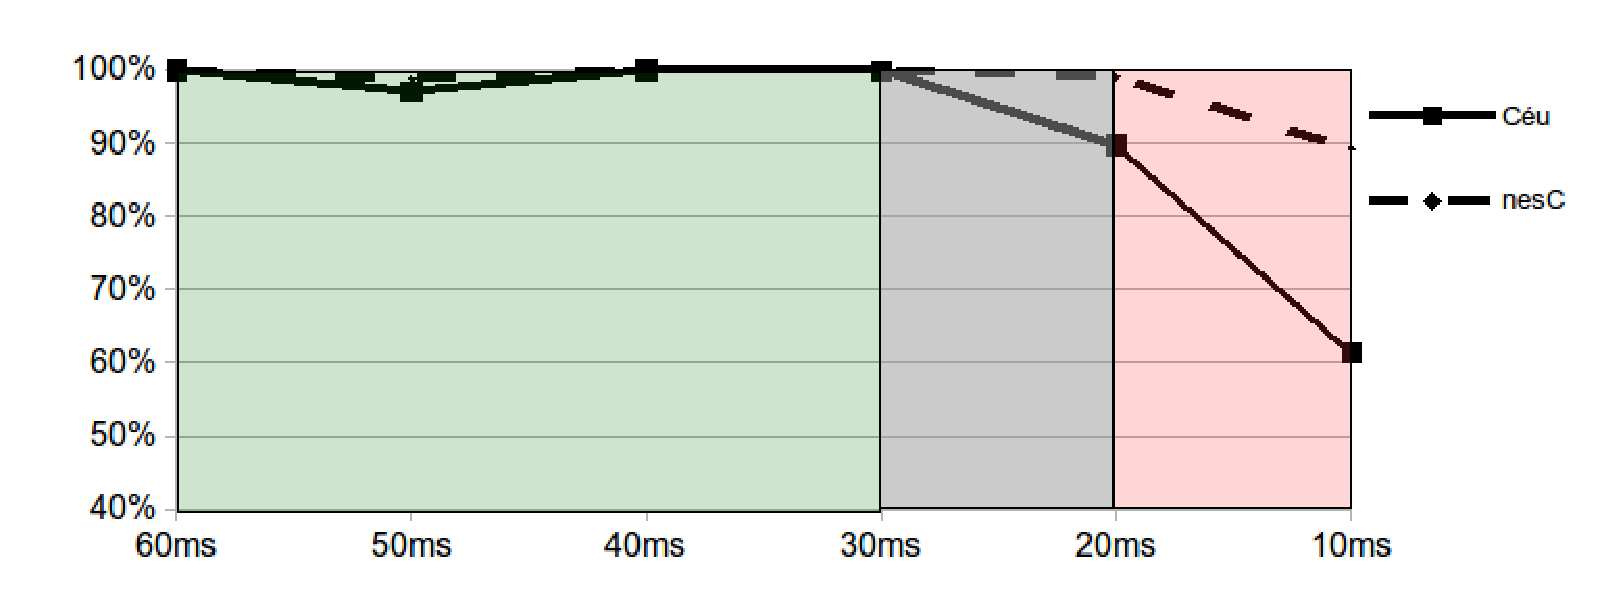
\includegraphics[width=\linewidth,clip=true,trim=35px 0px 10px 0px]{radio2}
\caption{  Percentage of received packets depending on the sending frequency.  
\newline
{\small %\textmd{
Each received packet is tied to a 8-ms operation.
\CEU is 100\% responsive up to a frequency of 30ms per packet.
}%}
\label{fig.radio2}
}
\end{figure}

% TODO: reaction times, measure or cite?

The overall conclusion from the experiments is that the radio driver in \CEU 
performs as well as the original driver in \emph{nesC} under high loads for 
programs with lengthy operations of up to 4ms, which is a reasonable time for 
control execution and simple processing.
%
The range between 6ms and 16ms offers opportunities for performing more complex 
operations, but also requires careful analysis and testing.
%
For instance, the last experiment shows that the \CEU driver can process in 
real time messages arriving every 33ms in sequence with a 8-ms operation.
%
%For operations over 64ms, neither \CEU or \emph{nesC} have real-time 
%responsiveness under high-loads.

Note that our experiments represent a ``stress-test'' scenario that is atypical 
to WSNs.
Protocols commonly use longer intervals between message transmissions together 
with mechanisms to avoid contention, such as randomized 
timers~\cite{wsn.trickle,wsn.ctp}.
Furthermore, WSNs are not subject to strict deadlines, being not classified as 
hard real-time systems~\cite{wsn.decade}.

\section{Battery consumption}
\label{sec.eval.batt}

Battery consumption is critical in WSNs, given that motes usually have no other 
source of energy and, in the case of being deployed in remote locations, cannot 
have the batteries replaced.

In order to evaluate battery consumption in \CEU in comparison to \emph{nesC}, 
we adapted the experiments of Section~\ref{sec.eval.radio}.
%
The parameters were adjusted to make the implementations in the two languages 
behave the same, i.e., the receiving node should receive the same amount of 
packets during the same period.

For the first experiment, we made each sending node transmit 75 messages 
during 150s, resulting in around 625 received packets (considering the 
losses) in the receiving mote, which also performs a 1-ms heavy activity 
every 1.5 seconds.
%
In this experiment, the CPU is idle most of the time and the battery is 
consumed by the radio hardware.
%
For the second experiment, we included a 2-ms heavy activity after every 
received packet, making the battery to be also consumed by the CPU.
%
Figure~\ref{fig.batt} shows the battery consumption (total and with active and 
idle CPU) for the two experiments and for both implementations.

\begin{figure*}[t]
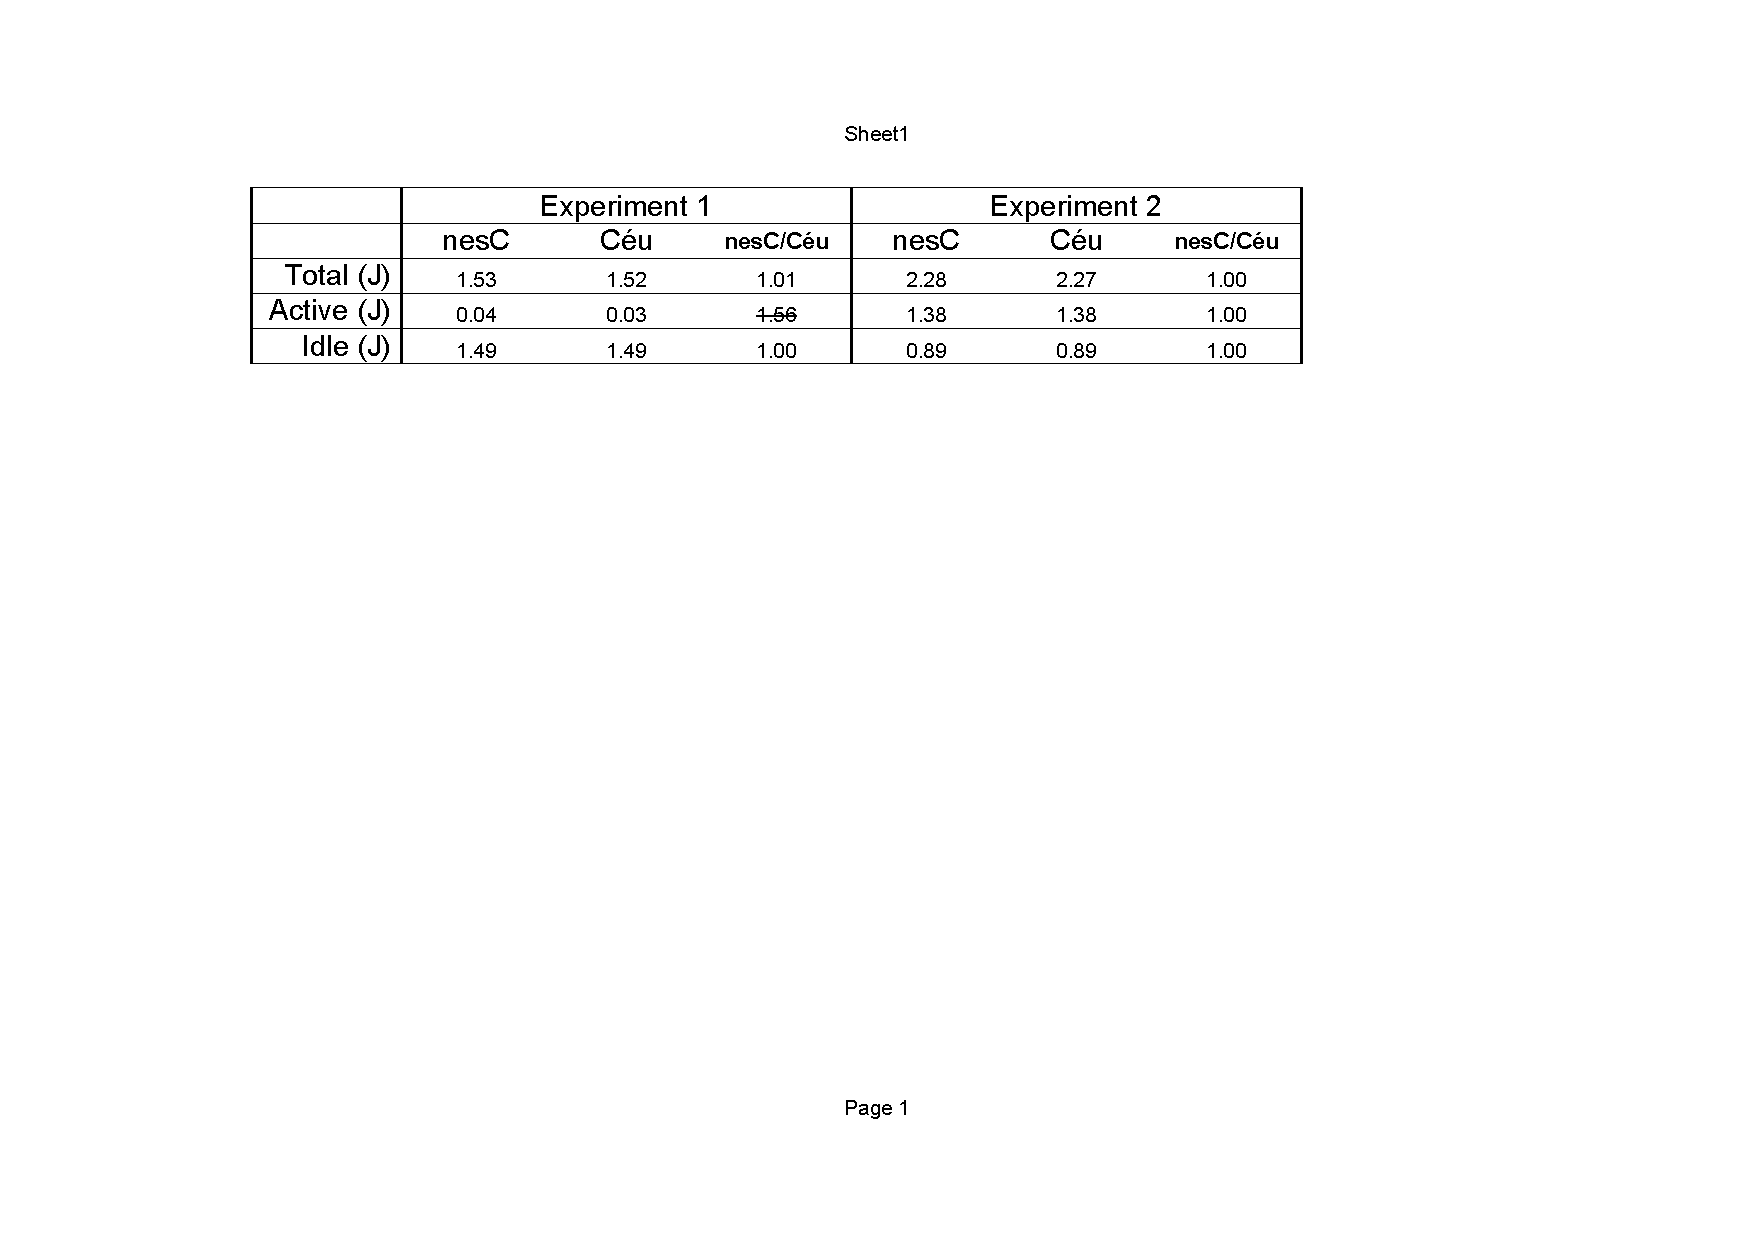
\includegraphics[width=\textwidth,clip=true,trim=120px 415px 210px 90px]{batt}
\caption{ Battery consumption for \emph{nesC} and \CEU in the two experiments.
\newline
{\small %\textmd{
The consumption line "Active" for the Experiment 1 is negligible, hence, the 
ratio between \emph{nesC} and \CEU should not be considered.
}%}
\label{fig.batt}
}
\end{figure*}

We did not expect a noticeable difference in battery usage between \CEU and 
\emph{nesC}, because, even considering the support for multiple lines of 
execution in \CEU, the compiler generates simple event-driven code in $C$, not 
requiring threads or complex runtime apparatus.
%
In fact, the results are virtually the same for both I/O and CPU-bound 
experiments.

\section{Discussion}

\CEU targets control-intensive applications and provides abstractions that can 
express program flow specifications concisely.
%
Our evaluation shows a considerable decrease in code size that comes from 
logical compositions of trails through the \code{par/or} and \code{par/and} 
constructs.
%
They handle startup and termination for trails seamlessly without extra 
programming efforts.
%
We believe that the small overhead in memory qualifies \CEU as a realistic 
option for constrained devices.
%
% TODO:
%Support for local variables did not lead to reduction in RAM, they and
%are and increase .
%
% TODO
%with overheads below 5\% and 10\%
%Some overhead in memory exists, but RAM is minimal and can be avoided XXX an 
%trackable
%inherent per-trail overhead.
%
%The overhead in ROM is below 10\% but has not .
%
%The main aspect of \CEU is to ensure that the high degree of concurrency in 
%WSNs does not pose safety threats to applications.
%
Furthermore, our broad safety analysis, encompassing all proposed concurrency 
mechanisms, ensures that the high degree of concurrency in WSNs does not pose 
safety threats to applications.
%
%Even with the restrictions that were needed to enable this analysis, \CEU was 
%shown to be expressive enough to imply in a decrease in code complexity for a 
%range of typical WSN applications.
%
%By restricting the expressiveness of the language, we could enable a broad 
%safety analysis in programs at compile time.
%The analysis encompasses all proposed concurrency mechanisms, such as parallel 
%compositions, first-class timers, and communication via events.
%
As a summary, the following safety properties hold for all programs that 
successfully compile in \CEU:

\begin{itemize}
\item Time-bounded reactions to the environment
        (Sections~\ref{sec.ceu.det}~and~\ref{sec.ceu.ints}).
\item Reliable weak and strong abortion among activities
        (Sections~\ref{sec.ceu.det}~and~\ref{sec.ceu.shared}).
\item No concurrency in accesses to shared variables
(Section~\ref{sec.ceu.shared}).
\item No concurrency in system calls sharing a resource
        (Section~\ref{sec.ceu.c}).
\item Finalization for blocks going out of scope
        (Section~\ref{sec.ceu.fins}).
\item Auto-adjustment for timers in sequence
        (Section~\ref{sec.ceu.wclocks}).
\item Synchronization for timers in parallel
        (Section~\ref{sec.ceu.wclocks}).
\end{itemize}

These properties are desirable in any application and are guaranteed as 
preconditions in \CEU by design.
Ensuring or even extracting these properties from less restricted languages 
requires significant manual analysis.

Even though the achieved expressiveness and overhead of \CEU meet the 
requirements of WSNs, its design imposes two inherent limitations:
the lack of dynamic loading which would forbid the static analysis,
and the lack of hard real-time guarantees.
%
Regarding the first limitation, dynamic features are already discouraged due to 
resource constraints.
For instance, even object-oriented languages targeting WSNs forbid dynamic 
allocation~\cite{wsn.flowtalk,wsn.virgil}.

To deal with the second limitation, which can be critical in the presence of 
lengthy computations, we can consider the following approaches:
(1) manually placing \code{pause} statements in unbounded loops;
(2) integrating \CEU with a preemptive system.
%
The first option requires the lengthy operations to be rewritten in \CEU using
\code{pause} statements so that other trails can be interleaved with them.
This option is the one recommended in many related work that provide a similar 
cooperative primitive (e.g. \code{pause}~\cite{esterel.primer}, 
\code{PT\_YIELD}~\cite{wsn.protothreads}, \code{yield}~\cite{wsn.sol}, 
\code{post}~\cite{wsn.nesc}).
%
Considering the second option, \CEU and preemptive threads are not mutually 
exclusive.
% and the second option is appealing to be explored in a future work.
For instance, TOSThreads~\cite{wsn.tosthreads} proposes a message-based 
integration with \emph{nesC} that is safe and matches the semantics of \CEU 
external events.

%%%%%%%%%%%%%%%%%%%%%%%%%%%%%%%%%%%%%%%%%%%%%%%%%%%%%%%%%%%%%%%%%%%%%%%%%%%%%%%

\begin{comment}

In order to evaluate the current implementation of \CEU{}, we performed initial
experiments in the domain of Wireless Sensor Networks%
\footnote{The complete source code for the evaluation can be found at \\
\url{http://www.ceu-lang.org/TR/\#exp1}.}.
Our goal is to compare \CEU{} with other languages implementations regarding 
two important aspects for WSNs: \emph{memory usage} and \emph{responsiveness}%
\footnote{Responsiveness is the ability of a system to promptly acknowledge 
high-priority requests (e.g. radio messages).}.

\textbf{Memory usage}

\newcommand{\dif}{{\small \CEU{}--\nesc{}}}
\newcommand{\s}[1]{{\small \textbf{#1}}}

%TODO: basestation_buffer

\begin{table}[t]\small
\begin{center}
\begin{tabular}{ | l | r | r | r | r | }
\hline
\multicolumn{2}{|c|}{}
           &          ROM &         RAM \\
\hline\hline
\multirow{3}{*}{Blink}
    & \nesc &  2048 bytes &    51 bytes \\
    & \CEU  &  5882 bytes &   168 bytes \\
    & \dif  &    \s{3834} &     \s{117} \\
\hline\hline
\multirow{3}{*}{Sense}
    & \nesc &  4366 bytes &    84 bytes \\
    & \CEU  &  8086 bytes &   195 bytes \\
    & \dif  &  \s{3720}   &     \s{111} \\
\hline\hline
\multirow{3}{*}{Client}
    & \nesc & 11838 bytes &   329 bytes \\
    & \CEU  & 15328 bytes &   482 bytes \\
    & \dif  &    \s{3490} &     \s{153} \\
\hline\hline
\multirow{3}{*}{Server}
    & \nesc & 14648 bytes &   373 bytes \\
    & \CEU  & 15686 bytes &   443 bytes \\
    & \dif  &    \s{1038} &      \s{70} \\
\hline
\end{tabular}
\end{center}
\caption{\CEU{} vs TinyOS: memory usage}
\label{tab:eval}
\end{table}

In the first experiment, we ported preexisting \nesc applications to \CEU.
We chose \nesc{} given its popularity in the context of WSNs, and because it is 
event based, consuming less memory than multithreaded languages.
By using preexisting applications in our experiment, we intend not to choose 
specific scenarios that favor one language or the other.

Table~\ref{tab:eval} shows the amount of ROM and RAM for the same applications 
written in \nesc{} and \CEU{}.
The third line for each application shows the difference for a given measure, 
for example: the Client application written in \CEU{} uses $3490$ more bytes 
than its \nesc{} counterpart.

Our experiment suggests that as application complexity grows, the memory 
footprint of \CEU{} becomes diluted, and the difference in consumption 
decreases, showing that \CEU{} is a viable alternative.

%TODO
%Note that \CEU{} already runs on top of \nesc{}, so in theory, the difference 
%should never , which already queues, extra mem we have no control

\textbf{Responsiveness}

\begin{table}[t]\small
\begin{center}
\begin{tabular}{ | l | l | c | c | }
\hline
\multicolumn{2}{|c|}{}
               & no comp. &    5 loops \\
\hline\hline
\multirow{2}{*}{1 sender}
    & MantisOS &  $23.2s$ &    $23.3s$ \\
    & \CEU     &  $23.3s$ &    $23.3s$ \\
\hline\hline
\multirow{2}{*}{2 senders}
    & MantisOS &  $19.8s$ &   $19.9s$ \\
    & \CEU     &  $12.3s$ &   $12.4s$ \\
\hline
\end{tabular}
\\
{\scriptsize\emph{(the measures are the average of three consecutive 
executions)}}
\caption{\CEU{} vs MantisOS: responsiveness}
\label{tab:resp}
\end{center}
\end{table}

In the second experiment, we measure how fast motes can answer radio requests 
when subjected to long computations.
We chose to compare \CEU{} with MantisOS~\cite{wsn.mantisos}, given that 
multithreaded systems perform better in this aspect \cite{wsn.comparison}.
Table~\ref{tab:resp} summarizes the results of this experiment, which is 
described next.

Initially, we created two simple applications that send and receive radio 
messages---with no processing in parallel---to measure how fast they exchange 
$3000$ messages without losses.
We varied the sending speed, and the fastest the receiving side could sustain 
without losses was around $7$ms for each message (coincidentally, in both 
implementations), resulting in $23$s for the entire process 
(\emph{``1~sender/no~comp.''} in Table~\ref{tab:resp}).

In order to evaluate the responsiveness of the receiving side, we changed it to 
also execute in parallel five infinite loops that run forever (to represent 
long computations).
In both \CEU{} and MantisOS implementations, the $3000$ messages were still 
received without losses, while the increase in the total receiving time was 
negligible
(\emph{``1~sender/5~loops''} in Table~\ref{tab:resp}).

In MantisOS, we had to change the priority of the receiving thread to be higher 
than the others.
In \CEU{} the receiving part (which is synchronous) already runs with higher 
priority than long computations (which run inside \emph{asyncs}).

In another test, we kept the single receiver and used two senders to measure 
how fast the receiving side receives $3000$ messages (now ignoring the losses) 
while running long computations in parallel.

Although \CEU{} performs better than MantisOS (probably due to TinyOS higher 
performance), our objective is to measure the \emph{increase} in the total time 
due to the long computations running in parallel.
Again the increase in time is negligible in both implementations.
(\emph{``2~senders''} in Table~\ref{tab:resp}).

From the second experiment, we conclude that \CEU{} is comparable to a 
multithreaded implementation in terms of responsiveness, both having nearly 
optimal behavior for the tests we performed.
Although not in the scope of this work, we asserted that, for all tests, both 
implementations performed a fair scheduling among long computations.

\end{comment}
